\documentclass[10pt,ngerman]{scrartcl}
\def\class{10}
\newcount\year
\year=2023
\newcount\nextyear
\nextyear=\number\year
\advance\nextyear by 1

%Variable for displaying solutions, if solution equals 1, they are displayed
\newcounter{DisplaySolution}
\setcounter{DisplaySolution}{0}

\usepackage[ngerman]{babel}
\usepackage{paralist}
\usepackage{multicol}
\usepackage[shortlabels]{enumitem}
\setlist[enumerate]{leftmargin=*}
\usepackage{amsmath,amssymb,wasysym}
\usepackage[final]{graphicx}
\usepackage{subcaption}
\usepackage{setspace}
\usepackage{picinpar}
\usepackage{siunitx}
\sisetup{
    mode=text,
    reset-text-family=false,
    reset-text-series=false,
    reset-text-shape=true,
    reset-math-version=false,
    propagate-math-font=true,
    text-family-to-math=true,
    text-series-to-math=true,
    output-decimal-marker = {,}, 
    group-separator = {}, 
    exponent-product = \cdot, 
    per-mode = fraction, 
    inter-unit-product = \cdot
}
\DeclareSIUnit\bar{bar}
\DeclareSIUnit\atm{atm}
\DeclareSIUnit\torr{torr}

\usepackage{icomma}
\usepackage[left=2.5cm,right=2.5cm,vmargin={3.2cm,2cm},headheight=100pt]{geometry}
\usepackage{fancybox}
\usepackage{fancyhdr}
\usepackage[version=3]{mhchem}
\usepackage{chemformula}
\usepackage{lastpage}
\usepackage{sectsty}
\usepackage{xcolor}
\usepackage{tabularx}
\usepackage{hyperref}

\usepackage{ifthen}

\usepackage{subfiles}

\usepackage{array}
\newcolumntype{L}[1]{>{\raggedright\arraybackslash}p{#1}}
\newcolumntype{C}[1]{>{\centering\arraybackslash}p{#1}}
\newcolumntype{R}[1]{>{\raggedleft\arraybackslash}p{#1}}

\usepackage{caption}
\usepackage{framed}
\usepackage{wrapfig}

\usepackage{multirow}

\definecolor{purple}{HTML}{9D2D72}
\sectionfont{\color{purple}\itshape}
\renewcommand*{\familydefault}{\sfdefault}
\setlength{\columnsep}{30pt}
\setlist[enumerate,1]{font=\itshape}

\usepackage{tikz}
\usetikzlibrary{arrows,positioning,angles,quotes,calc,shapes.geometric,babel}
\tikzset{
    >=stealth',
    punkt/.style={
           rectangle,
           rounded corners,
           draw=black, very thick,
           text width=6.5em,
           minimum height=2em,
           text centered},
    pil/.style={
           ->,
           thick,
           shorten <=2pt,
           shorten >=2pt,}
}
\usepackage{pgfplots}
\pgfplotsset{compat=1.5}

\usepackage{float}
\usepackage[nomessages]{fp}
\usepackage{bm}

\newcommand{\choiceold}[5]{
        \par
        \renewcommand{\arraystretch}{1.1}
        {\setlength{\tabcolsep}{2pt}
        \begin{tabular}{*{5}{@{}|>{\hspace{2pt}}p{0.19\textwidth}<{\hspace{2pt}}}|}\hline \itshape
        (a)~#1 & (b)~#2 & (c)~#3 & (d)~#4  & (e)~#5\\\hline
        \end{tabular}}
}

\newcommand{\choice}[5]{        
        \par
        \renewcommand{\arraystretch}{1.1}
        {\setlength{\tabcolsep}{2pt}
        \begin{tabular}{|p{0.179\textwidth} p{0.001\textwidth}|p{0.179\textwidth} p{0.001\textwidth}|p{0.179\textwidth} p{0.001\textwidth}|p{0.179\textwidth} p{0.001\textwidth}|p{0.179\textwidth} p{0.001\textwidth}|}\hline 
        (a)~#1 & & (b)~#2 & & (c)~#3 & & (d)~#4 & & (e)~#5 &\\\hline
        \end{tabular}}
}

\usepackage{marginnote}

\usepackage[most]{tcolorbox}
\usepackage{lipsum}

\makeatletter
\begingroup
\toks0=\expandafter{\@settodim{#1}{#2}{#3}}
\edef\x{\endgroup
  \long\def\noexpand\@settodim##1##2##3{\the\toks0 }}\x
\makeatother

\newcommand{\emptybox}{{\Large \Square}}
\newcommand{\checkedbox}{{\Large \XBox}}

\newcounter{start}
\addtocounter{start}{2100}
\addtocounter{start}{\class}

\newcommand{\g}{\gram}
\newcommand{\ml}{\milli\liter}
\renewcommand{\c}{\celsius}
\newcommand{\gmol}{\gram\per\mol}
\newcommand{\gcm}{\gram\per\cubic\centi\meter}
\newcommand{\kpa}{\kilo\pascal}
\renewcommand{\l}{\liter}
\fancyhf{}
\fancyhead[L]{\framebox[2.5cm]{\Large\bfseries 24\class -\hfill}\vfill}
\fancyhead[C]{\Large \textbf{\glqq{}Chemie -- die stimmt!\grqq{} {\number\year}/{\number\nextyear}\\
\ifnum \value{DisplaySolution}=1
    Musterlösungen
\else
    Aufgabenblatt
\fi
\\4. Runde -- Klasse \class}}
\fancyhead[R]{\includegraphics[height=2cm]{Format_Material/CDS_Logo_Map_verbessert.eps}}
\fancyfoot[L]{\thepage\ von \pageref*{LastPage}}
\pagestyle{fancy}

\setlength{\parindent}{0pt}
\addto\captionsngerman{\renewcommand{\figurename}{Abb.}}

\newcommand{\answer}[1]{
	\setalph
	\stepcounter{ex}
    {\noindent \theex}
	\nopagebreak
	\begin{framed}
		\vspace*{#1}
	\end{framed}
}

\newcommand{\answern}[1]{
	\begin{framed}
		\vspace*{#1}
	\end{framed}
}

\usepackage{calc}
\newlength{\someheight}
\newlength{\boxheight}
\newlength{\remainingheight}

\newcommand{\solution}[2]{
    \settototalheight{\someheight}{\vbox{#1}}
    \setlength{\boxheight}{#2}
    \ifnum \value{DisplaySolution}=1
        \begin{framed}
            \textcolor{red}{#1}
            \ifdim\boxheight>\someheight
                \setlength{\remainingheight}{\boxheight-\someheight}
                \vspace*{\remainingheight}
            \else
                \textcolor{red}{!!!DU KEK!!!}
            \fi
        \end{framed}
    \else
        \begin{framed}
            \vspace*{#2}
        \end{framed}
    \fi
}

\newcommand{\solutiontext}[2]{
    \ifnum \value{DisplaySolution}=1
        \textcolor{red}{#1}
    \else
        #2
    \fi
}

\newcommand{\enumaufgabe}[1]{
\begin{enumerate}[a), resume]
\itshape
\item {#1}
\end{enumerate}
}

\newcommand{\enumersteaufgabe}[1]{
\begin{enumerate}[a)]
\itshape
\item {#1}
\end{enumerate}
}

\newcommand{\operator}[1]{\underline{\textbf{#1}}}

\newcommand{\enumMC}[1]{
\begin{enumerate}[1., resume]
\itshape
\item {#1}
\end{enumerate}
}

\ifthenelse{\value{DisplaySolution}=1}{%
  \definecolor{answercolor}{rgb}{1,0,0}%red
}{%
  \definecolor{answercolor}{rgb}{0,0,0}%black
}

\newcommand{\solutionwrapper}[1]{
    \settototalheight{\someheight}{\vbox{#1}}
    \ifnum \value{DisplaySolution}=1
        #1
    \else
        \vspace*{\someheight}
    \fi
}

% Define a custom tcolorbox environment for answer boxes
\tcbuselibrary{breakable}
\newtcolorbox{answerbox}[1][]{%
  enhanced,
  breakable,
  colframe=black,
  colback=white,
  coltext=answercolor,
  width=\textwidth,
  before skip=10pt,
  after skip=10pt,
  #1
}

\usepackage{expl3,xparse}
\ExplSyntaxOn
\box_new:N \l_mypkg_box
\int_new:N \l_mypkg_cleanup_int
\DeclareDocumentCommand{\hideit}{O{1}+m}
  {
    \tex_setbox:D \l_mypkg_box \tex_vbox:D
      {
        #2\par
        \dim_zero:N \tex_baselineskip:D
        \dim_zero:N \tex_lineskip:D
        \dim_zero:N \tex_lineskiplimit:D
        \int_set:Nn \l_mypkg_cleanup_int {#1}
        \mypkg_dismantle_loop:
      }
    \tex_unvbox:D \l_mypkg_box
  }
\cs_new_protected:Npn \mypkg_dismantle_loop:
  {
    \prg_replicate:nn { \l_mypkg_cleanup_int }
      {
        \skip_if_eq:nnT { \tex_lastskip:D } { \c_zero_skip } { \tex_unskip:D }
        \dim_compare:nT { \tex_lastkern:D = \c_zero_dim } { \tex_unkern:D }
        \int_compare:nT { \tex_lastpenalty:D = \c_zero } { \tex_unpenalty:D }
      }
    \skip_if_eq:nnTF { \tex_lastskip:D } { \c_zero_skip }
      {
        \dim_compare:nTF { \tex_lastkern:D = \c_zero_dim }
          {
            \int_compare:nTF { \tex_lastpenalty:D = \c_zero }
              {
                \box_set_to_last:N \l_mypkg_box
                \box_if_empty:NF \l_mypkg_box
                  { \mypkg_dismantle_box: }
              }
              { \mypkg_dismantle_penalty: }
          }
          { \mypkg_dismantle_kern: }
      }
      { \mypkg_dismantle_skip: }
  }
\cs_new_protected:Npn \mypkg_dismantle_skip:
  { \mypkg_dismantle_aux:nN { \tex_vskip:D \skip_use:N \tex_lastskip:D } \tex_unskip:D }
\cs_new_protected:Npn \mypkg_dismantle_kern:
  { \mypkg_dismantle_aux:nN { \tex_kern:D \dim_use:N \tex_lastkern:D } \tex_unkern:D }
\cs_new_protected:Npn \mypkg_dismantle_penalty:
  { \mypkg_dismantle_aux:nN { \tex_penalty:D \int_use:N \tex_lastpenalty:D } \tex_unpenalty:D }
\cs_new_protected:Npn \mypkg_dismantle_box:
  { \mypkg_dismantle_aux:nN { \tex_vbox:D to \dim_eval:n { \box_ht:N \l_mypkg_box + \box_dp:N \l_mypkg_box } { } } \scan_stop: }
\cs_new_protected:Npn \mypkg_dismantle_aux:nN #1#2
  {
    \use:x
      {
        #2
        \mypkg_dismantle_loop:
        #1 \scan_stop:
      }
  }
\ExplSyntaxOff
\fancyhead[L]{\framebox[2.5cm]{\Large\bfseries 2410-\hfill}\vfill}

\sisetup{detect-none = true}
\sisetup{detect-weight = true}

\begin{document}

\begin{center}
    \Large \textbf{Hinweise zur Klausur}
\end{center}
Achte darauf, dass du auf jedem Blatt auf dem Antwortbogen deine Startnummer gut lesbar im dafür vorgesehenen Kästchen notierst. Lies dir zu Beginn alle Aufgaben gründlich durch. Viel Erfolg!

\begin{center}
    \Large \textbf{Periodensystem}
    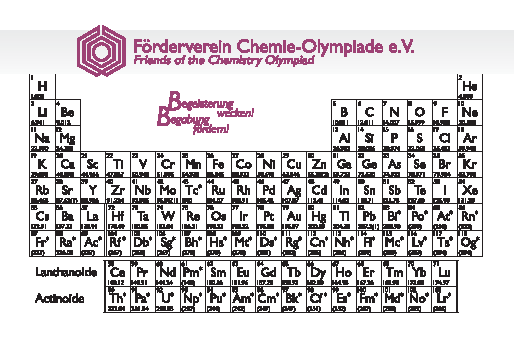
\includegraphics[page=1, scale=2.5, angle=270]{Format_Material/PSE.pdf}
\end{center}

\newpage
\section*{Formelsammlung}
\subsection*{wichtige chemische und physikalische Konstanten}
\begin{table}[H]
\renewcommand{\arraystretch}{1.3}
    \begin{tabular}{p{7cm} l}
        Elementarladung &  $e = \SI{1.602176e-19}{\coulomb}$\\
        Universelle Gaskonstante & $R = \SI{8,314456}{\joule\per\mol\per\kelvin}$\\
        Avogadro-Konstante & $N_\mathrm{A} = \SI{6,0221e23}{\per\mol}$\\
        Faraday Konstante & $F = \SI{96485,309}{\coulomb\per\mol}$\\
        Atomare Masseneinheit & $u =$ \SI{1,660539e-27}{\kilo\gram}\\
        Planck'sches Wirkungsquantum & $h = \SI{6.62607015E-34}{\joule\second}$\\
        Lichtgeschwindigkeit & $c = $ \SI{2.99792458e8}{\meter\per\second}
    \end{tabular}
\end{table}

\subsection*{Allgemeine Gleichungen}

\begin{table}[H]
\renewcommand{\arraystretch}{1.3}
    \begin{tabular}{p{7cm} l}
       ideales Gasgesetz & $p V = n R T$\\
       radioaktives Zerfallsgesetz & $N(t) = N(0) e^{-k t} = N(0) e^{-\frac{\ln 2}{T_{1/2}} t}$\\
    \end{tabular}
\end{table}

\subsection*{Gleichgewichte}

\begin{table}[H]
\renewcommand{\arraystretch}{1.3}
    \begin{tabular}{p{7cm} l}
       Massenwirkungsgesetz & $K_\mathrm{c} = \frac{c(\mathrm{C})^c \cdot c(\mathrm{D})^d \cdot \dots}{c(\mathrm{A})^a \cdot c(\mathrm{B})^b \cdot \dots}$\\
       Säure-Base-Gleichgewichte & $K_\mathrm{S} = \frac{c(\mathrm{H^+}) \cdot c(\mathrm{A^-})}{c(\mathrm{HA}) \cdot c_0}$\\
       & $K_\mathrm{B} = \frac{c(\mathrm{HB^+}) \cdot c(\mathrm{OH^-})}{c(\mathrm{B})\cdot  c_0}$\\
       pH-Wert & $\mathrm{pH} = - \log \frac{c(\mathrm{H^+})}{c_0}$\\
       Henderson-Hasselbalch & $\mathrm{pH} = \mathrm{p}K_\mathrm{S} + \log \frac{c(\ce{A-})}{c(\ce{HA})}$\\
    \end{tabular}
\end{table}

\subsection*{Thermodynamik und Elektrochemie}

\begin{table}[H]
\renewcommand{\arraystretch}{1.3}
    \begin{tabular}{p{7cm} l}
       Gibbs-Helmholtz-Gleichung & $\Delta G_\mathrm{R}^\circ = \Delta H_\mathrm{R}^\circ - T \Delta S_\mathrm{R}^\circ$\\
      Gibbs-Energie und Gleichgewichtskonstante & $\Delta G_\mathrm{R}^\circ = - R T \ln K$\\
       Faradaysches Gesetz & $Q = I \cdot t = z \cdot n \cdot F$
    \end{tabular}
\end{table}

\newpage

\section*{Multiple Choice}

Entscheide für \operator{jede} der Aussagen durch \operator{Ankreuzen}, ob sie richtig oder falsch ist.  Pro Frage können keine negativen Punkte erhalten werden. Unabhängig von der Formulierung der Fragestellung können auch mehrere Antworten richtig sein.



\renewcommand{\arraystretch}{1.2}

%Beispiel:
\begin{comment}
\enumMC{Aufgabe}
\begin{tabularx}{\textwidth}{|X|C{1.5cm}|C{1.5cm}|}\hline
    & wahr & falsch\\\hline
    Wahr & \solutiontext{\checkedbox}{\emptybox} & \emptybox \\\hline
    Falsch & \emptybox & \solutiontext{\checkedbox}{\emptybox} \\\hline
\end{tabularx}
\end{comment}
\enumMC{Welche Zusammensetzung aus physikalischen Größen ergibt eine Energie als Ergebnis? 
($l$ ist die Länge, $E$ die Energie, $P$ die Leistung, $t$ die Zeit, $\rho$ die Dichte, $g$ die Fallbeschleunigung, $H$ die Enthalpie, $V$ das Volumen, $R$ die Gaskonstante, $T$ die Temperatur, $M$ die molare Masse und $m$ die Masse)
}
\begin{tabularx}{\textwidth}{|X|C{1.5cm}|C{1.5cm}|}\hline
    & wahr & falsch\\\hline
    $(\gamma-1)\cdot mc^2$ & \solutiontext{\checkedbox}{\emptybox} & \emptybox \\\hline
    $P \cdot l \cdot c^{-1}$  & \solutiontext{\checkedbox}{\emptybox} & \emptybox \\\hline
    $\rho \cdot g \cdot l \cdot V$ & \solutiontext{\checkedbox}{\emptybox} & \emptybox \\\hline
    $p\cdot V^{\kappa}$  & \emptybox & \solutiontext{\checkedbox}{\emptybox} \\\hline
    $l^2 \cdot m \cdot t^{-1}$ & \emptybox & \solutiontext{\checkedbox}{\emptybox} \\\hline
\end{tabularx}

\enumMC{Welche der folgenden Moleküle ist gewinkelt?}
\begin{tabularx}{\textwidth}{|X|C{1.5cm}|C{1.5cm}|}\hline
    & wahr & falsch\\\hline
    \ce{SO2}  & \solutiontext{\checkedbox}{\emptybox} & \emptybox \\\hline
    \ce{H2O}  & \solutiontext{\checkedbox}{\emptybox} & \emptybox \\\hline
    \ce{CO2} & \emptybox & \solutiontext{\checkedbox}{\emptybox} \\\hline
    \ce{HOF}  & \solutiontext{\checkedbox}{\emptybox} & \emptybox \\\hline
    \ce{NO2-} & \solutiontext{\checkedbox}{\emptybox} & \emptybox \\\hline
\end{tabularx}


\enumMC{Welche der folgenden Moleküle ist trigonal-pyramidal?}
\begin{tabularx}{\textwidth}{|X|C{1.5cm}|C{1.5cm}|}\hline
    & wahr & falsch\\\hline
    \ce{NH3} & \solutiontext{\checkedbox}{\emptybox} & \emptybox \\\hline
    \ce{ClF3} & \emptybox & \solutiontext{\checkedbox}{\emptybox} \\\hline
    \ce{PCl3} & \solutiontext{\checkedbox}{\emptybox} & \emptybox \\\hline
    \ce{BF3} & \emptybox & \solutiontext{\checkedbox}{\emptybox} \\\hline
    \ce{NO3-} & \emptybox & \solutiontext{\checkedbox}{\emptybox} \\\hline
\end{tabularx}






\enumMC{Eine \SI{5}{\gram} schwere Probe eines radioaktiven Materials besitzt eine Halbwertszeit von \SI{10}{\hour}. Wie lange dauert es, bis nur noch \SI{1}{\gram} der ursprünglichen Substanz übrig ist?}
\begin{tabularx}{\textwidth}{|X|C{1.5cm}|C{1.5cm}|}\hline
    \SI{23,2}{\hour} & \solutiontext{\checkedbox}{\emptybox} & \emptybox \\\hline
    \SI{6,99}{\hour} & \emptybox & \solutiontext{\checkedbox}{\emptybox} \\\hline
    \SI{16,1}{\hour} & \emptybox & \solutiontext{\checkedbox}{\emptybox} \\\hline
    \SI{419,4}{\minute} & \emptybox & \solutiontext{\checkedbox}{\emptybox} \\\hline
    \SI{0,387}{\minute} & \emptybox & \solutiontext{\checkedbox}{\emptybox} \\\hline
\end{tabularx}

\enumMC{Welche der nachfolgend genannten Modifikationen des Phosphors sind bekannt?}


\begin{tabularx}{\textwidth}{|X|C{1.5cm}|C{1.5cm}|}\hline
    & wahr & falsch\\\hline
    violetter Phosphor & \solutiontext{\checkedbox}{\emptybox} & \emptybox \\\hline
    schwarzer Phosphor & \solutiontext{\checkedbox}{\emptybox} & \emptybox \\\hline
    weißer Phosphor & \solutiontext{\checkedbox}{\emptybox} & \emptybox \\\hline
    roter Phosphor & \solutiontext{\checkedbox}{\emptybox} & \emptybox \\\hline
    grüner Phosphor & \emptybox & \solutiontext{\checkedbox}{\emptybox} \\\hline
\end{tabularx}

\newpage

\enumMC{Welches Ion hat einen größeren Radius als \ce{Mg^2+}?}
\begin{tabularx}{\textwidth}{|X|C{1.5cm}|C{1.5cm}|}\hline
    & wahr & falsch\\\hline
    \ce{Al^3+} & \emptybox & \solutiontext{\checkedbox}{\emptybox} \\\hline
    \ce{He^2+} & \emptybox & \solutiontext{\checkedbox}{\emptybox} \\\hline
    \ce{Li+} & \solutiontext{\checkedbox}{\emptybox} & \emptybox \\\hline
    \ce{F-} & \solutiontext{\checkedbox}{\emptybox} & \emptybox \\\hline
    \ce{H-} & \solutiontext{\checkedbox}{\emptybox} & \emptybox \\\hline
\end{tabularx}

\enumMC{Welche Dichte besitzt Wasserstoffgas bei \SI{1}{\bar} und \SI{25}{\celsius}?}
\begin{tabularx}{\textwidth}{|X|C{1.5cm}|C{1.5cm}|}\hline
    & wahr & falsch\\\hline
    \SI{0,041}{\gram\per\liter} & \emptybox & \solutiontext{\checkedbox}{\emptybox} \\\hline
    \SI{0,081}{\gram\per\liter} & \solutiontext{\checkedbox}{\emptybox} & \emptybox \\\hline
    {\SI{0,093}{\gram\per\liter}} & \emptybox & \solutiontext{\checkedbox}{\emptybox} \\\hline
    {\SI{0,041}{\kilo\gram\per\cubic\meter}} & \emptybox & \solutiontext{\checkedbox}{\emptybox} \\\hline{\SI{0,081}{\kilo\gram\per\cubic\meter}} & \solutiontext{\checkedbox}{\emptybox} & \emptybox \\\hline
\end{tabularx}


\enumMC{Welche Reaktionen laufen an Kathode oder Anode bei der Elektrolyse einer wässrigen Lithiumsulfat-Lösung ab?}
\begin{tabularx}{\textwidth}{|X|C{1.5cm}|C{1.5cm}|}\hline
& wahr & falsch\\\hline
    \ce{Li+ + e- -> Li}& \emptybox & \solutiontext{\checkedbox}{\emptybox} \\\hline
    \ce{2H3O+ + 2e- -> 2H2O + H2}& \solutiontext{\checkedbox}{\emptybox} & \emptybox \\\hline
    \ce{SO2^{2-} -> SO2 + 2e-}& \emptybox & \solutiontext{\checkedbox}{\emptybox} \\\hline
    \ce{SO4^{2-} -> SO3 + 2e- + 0,5O2}& \emptybox & \solutiontext{\checkedbox}{\emptybox} \\\hline
    \ce{2OH- -> H2O + 0,5O2 + 2e-}& \solutiontext{\checkedbox}{\emptybox} & \emptybox \\\hline

\end{tabularx}





\enumMC{Zur Oxidation von \SI{0,1}{\mole} eines organischen Moleküls der Form \ce{C3H_yO_x} werden von einem Überschuss \ce{CrO3} \SI{26,664}{\gram} verbraucht. Dabei entsteht das Produkt der Form \ce{C3H_nO_i}. Welche Aussagen bezüglich jeder möglichen Verbindung \ce{C3H_yO_x} stimmen? \\Hinweis: Es gibt mehrere mögliche Verbindungen, die die Vorraussetzungen erfüllen.}
\begin{tabularx}{\textwidth}{|X|C{1.5cm}|C{1.5cm}|}\hline
& wahr & falsch\\\hline
x ist immer größer als 2 & \emptybox & \solutiontext{\checkedbox}{\emptybox} \\\hline
y ist immer größer als 6 & \emptybox & \solutiontext{\checkedbox}{\emptybox} \\\hline
y ist kleiner als 8 & \emptybox & \solutiontext{\checkedbox}{\emptybox} \\\hline
Es gibt keine mögliche Verbindung mit zwei Doppelbindungen. & \solutiontext{\checkedbox}{\emptybox} & \emptybox \\\hline
Bei allen Verbindungen handelt es sich um Alkohole.& \emptybox & \solutiontext{\checkedbox}{\emptybox} \\\hline

\end{tabularx}

\enumMC{Welche der folgenden Verbindungen hat mehr Heteroatome als \ce{C}-Atome?}
\begin{tabularx}{\textwidth}{|X|C{1.5cm}|C{1.5cm}|}\hline
& wahr & falsch\\\hline
Ameisensäure & \solutiontext{\checkedbox}{\emptybox} & \emptybox \\\hline
Formaldehyd & \emptybox & \solutiontext{\checkedbox}{\emptybox} \\\hline
Trichlorethanol & \solutiontext{\checkedbox}{\emptybox} & \emptybox \\\hline
Methyltrinitrobenzen & \solutiontext{\checkedbox}{\emptybox} & \emptybox \\\hline
Aminopropansäure & \emptybox & \solutiontext{\checkedbox}{\emptybox} \\\hline
\end{tabularx}

\newpage

\enumMC{Welche der folgenden Elemente hat eine höhere Elektronegativität (Pauling-Skala) als \ce{H}?}
\begin{tabularx}{\textwidth}{|X|C{1.5cm}|C{1.5cm}|}\hline
& wahr & falsch\\\hline
\ce{C} & \solutiontext{\checkedbox}{\emptybox} & \emptybox \\\hline
\ce{Pb} & \emptybox & \solutiontext{\checkedbox}{\emptybox} \\\hline
\ce{I} & \solutiontext{\checkedbox}{\emptybox} & \emptybox \\\hline
\ce{Au} & \solutiontext{\checkedbox}{\emptybox} & \emptybox \\\hline
\ce{Fr} & \emptybox & \solutiontext{\checkedbox}{\emptybox} \\\hline

\end{tabularx}

\enumMC{Welche der folgenden Elemente kommt in der Oxidationsstufe +3 vor?}
\begin{tabularx}{\textwidth}{|X|C{1.5cm}|C{1.5cm}|}\hline
& wahr & falsch\\\hline
    \ce{N} & \solutiontext{\checkedbox}{\emptybox} & \emptybox \\\hline
    \ce{Co} & \solutiontext{\checkedbox}{\emptybox} & \emptybox \\\hline
    \ce{Ti} & \solutiontext{\checkedbox}{\emptybox} & \emptybox \\\hline
    \ce{H} & \emptybox & \solutiontext{\checkedbox}{\emptybox} \\\hline
    \ce{Pb} & \emptybox & \solutiontext{\checkedbox}{\emptybox} \\\hline
\end{tabularx}




\enumMC{Welche der folgenden Verbindung ist in wässriger Lösung farbig?}
\begin{tabularx}{\textwidth}{|X|C{1.5cm}|C{1.5cm}|}\hline
& wahr & falsch\\\hline
\ce{Al2(SO4)3} & \emptybox & \solutiontext{\checkedbox}{\emptybox} \\\hline
\ce{FeCl3} & \solutiontext{\checkedbox}{\emptybox} & \emptybox \\\hline
\ce{MnS} & \solutiontext{\checkedbox}{\emptybox} & \emptybox \\\hline
\ce{CuSO4} & \solutiontext{\checkedbox}{\emptybox} & \emptybox \\\hline
\ce{ZnCl2} & \emptybox & \solutiontext{\checkedbox}{\emptybox} \\\hline

\end{tabularx}

\enumMC{Was ist der pH-Wert einer 0,3 molaren Salzsäure-Lösung?}
\begin{tabularx}{\textwidth}{|X|C{1.5cm}|C{1.5cm}|}\hline
    & wahr & falsch\\\hline
    -2,74& \emptybox & \solutiontext{\checkedbox}{\emptybox} \\\hline
    -0,52& \emptybox & \solutiontext{\checkedbox}{\emptybox} \\\hline
    0,52& \solutiontext{\checkedbox}{\emptybox} & \emptybox \\\hline
    1,57& \emptybox & \solutiontext{\checkedbox}{\emptybox} \\\hline
    3,26& \emptybox & \solutiontext{\checkedbox}{\emptybox} \\\hline
\end{tabularx}

\enumMC{Welche der folgenden Säuren wirkt stark oxidierend?}
\begin{tabularx}{\textwidth}{|X|C{1.5cm}|C{1.5cm}|}\hline
    & wahr & falsch\\\hline
    Salpetersäure& \solutiontext{\checkedbox}{\emptybox} & \emptybox \\\hline
    Oxalsäure& \emptybox & \solutiontext{\checkedbox}{\emptybox} \\\hline
    Borsäure& \emptybox & \solutiontext{\checkedbox}{\emptybox} \\\hline
    Chlorsäure& \solutiontext{\checkedbox}{\emptybox} & \emptybox \\\hline
    Peroxomonoschwefelsäure& \solutiontext{\checkedbox}{\emptybox} & \emptybox \\\hline
\end{tabularx}

\enumMC{Bei welchen der folgenden Möglichkeiten sind die Gase nach aufsteigender Dichte geordnet?}
\begin{tabularx}{\textwidth}{|X|C{1.5cm}|C{1.5cm}|}\hline
    & wahr & falsch\\\hline
    \ce{N2}<\ce{O2}<\ce{O3}<\ce{CO2}<\ce{Ar} & \emptybox & \solutiontext{\checkedbox}{\emptybox} \\\hline
    \ce{Ne}<\ce{N2}<\ce{F2}<\ce{Ar}<\ce{O3} & \solutiontext{\checkedbox}{\emptybox} & \emptybox \\\hline
    \ce{O2}<\ce{F2}<\ce{Cl2}<\ce{Ar}<\ce{CO2} & \emptybox & \solutiontext{\checkedbox}{\emptybox} \\\hline
    \ce{N2}<\ce{O2}<\ce{F2}<\ce{Ar}<\ce{Cl2} & \solutiontext{\checkedbox}{\emptybox} & \emptybox \\\hline
    \ce{F2}<\ce{N2}<\ce{CO2}<\ce{Ar}<\ce{Cl2} & \emptybox & \solutiontext{\checkedbox}{\emptybox} \\\hline
\end{tabularx}

\enumMC{Welche der folgenden Aussagen über das chemische Gleichgewicht sind korrekt?}
\begin{tabularx}{\textwidth}{|X|C{1.5cm}|C{1.5cm}|}\hline
    & wahr & falsch\\\hline
    Der Reaktionsquotient $Q$ entspricht während der Reaktion immer der Gleichgewichtskonstante $K$.& \emptybox & \solutiontext{\checkedbox}{\emptybox} \\\hline
    Eine Erhöhung der Eduktkonzentration verringert der Wert von $K$.& \emptybox & \solutiontext{\checkedbox}{\emptybox} \\\hline
    Jede Reaktion besitzt ein chemisches Gleichgewicht.& \emptybox & \solutiontext{\checkedbox}{\emptybox} \\\hline
    $K$ ist von der Temperatur abhängig.& \solutiontext{\checkedbox}{} & \emptybox \\\hline
    $K$ ist unabhängig von den Geschwindigkeitskonstanten $k$ der Hin- und Rückreaktion.& \emptybox & \solutiontext{\checkedbox}{\emptybox}\\\hline
\end{tabularx}

\enumMC{Welche der folgenden Teilchen können bei einem radioaktiven Zerfall entstehen?}
\begin{tabularx}{\textwidth}{|X|C{1.5cm}|C{1.5cm}|}\hline
    & wahr & falsch\\\hline
    Elektronen& \solutiontext{\checkedbox}{\emptybox} & \emptybox \\\hline
    Neutrinos& \solutiontext{\checkedbox}{\emptybox} & \emptybox \\\hline
    \ce{^4He}-Atome& \emptybox & \solutiontext{\checkedbox}{\emptybox} \\\hline
    Positronen& \solutiontext{\checkedbox}{\emptybox} & \emptybox \\\hline
    Albinos& \emptybox & \solutiontext{\checkedbox}{\emptybox} \\\hline
\end{tabularx}

\enumMC{Welcher der folgenden Kerne ist der stabilste?}
\begin{tabularx}{\textwidth}{|X|C{1.5cm}|C{1.5cm}|}\hline
    & wahr & falsch\\\hline
    \ce{^{52}Cr}& \emptybox & \solutiontext{\checkedbox}{\emptybox} \\\hline
    \ce{^{55}Mn}& \emptybox & \solutiontext{\checkedbox}{\emptybox} \\\hline
    \ce{^{58}Fe}& \solutiontext{\checkedbox}{\emptybox} & \emptybox \\\hline
    \ce{^{58}Ni}& \emptybox & \solutiontext{\checkedbox}{\emptybox} \\\hline
    \ce{^{59}Co}& \emptybox & \solutiontext{\checkedbox}{\emptybox} \\\hline
\end{tabularx}

\enumMC{Welche der folgenden Metalle scheiden sich an einer Zinkplatte ab, wenn man diese in die entsprechende Metallsalz-Lösung stellt?}
\begin{tabularx}{\textwidth}{|X|C{1.5cm}|C{1.5cm}|}\hline
    & wahr & falsch\\\hline
    Kupfer& \solutiontext{\checkedbox}{\emptybox} & \emptybox \\\hline
    Blei& \solutiontext{\checkedbox}{\emptybox} & \emptybox \\\hline
    Aluminium& \emptybox & \solutiontext{\checkedbox}{\emptybox} \\\hline
    Eisen& \solutiontext{\checkedbox}{\emptybox} & \emptybox \\\hline
    Cobalt& \solutiontext{\checkedbox}{\emptybox} & \emptybox \\\hline
\end{tabularx}

\enumMC{Welche der folgenden Aussagen über den Halbäquivalenzpunkt sind korrekt?}
\begin{tabularx}{\textwidth}{|X|C{1.5cm}|C{1.5cm}|}\hline
    & wahr & falsch\\\hline
    $\mathrm{pH}=\mathrm{p}K_\mathrm{S}$ & \solutiontext{\checkedbox}{\emptybox} & \emptybox \\\hline
    Der Halbäquivalenzpunkt kann nie in der Titrationskurve erkannt werden.& \emptybox & \solutiontext{\checkedbox}{\emptybox} \\\hline
    $\mathrm{pH}=3,75$& \emptybox & \solutiontext{\checkedbox}{\emptybox} \\\hline
    $\mathrm{pH}=\frac{1}{2}\mathrm{p}K_\mathrm{S}$& \emptybox & \solutiontext{\checkedbox}{\emptybox} \\\hline
    $[\ce{HA}]=[\ce{A^-}]$& \solutiontext{\checkedbox}{\emptybox} & \emptybox \\\hline
\end{tabularx}

\enumMC{Welche der folgenden Aussagen über Phenol (Benzenol) sind korrekt?}
\begin{tabularx}{\textwidth}{|X|C{1.5cm}|C{1.5cm}|}\hline
    & wahr & falsch\\\hline
    Phenol ist elektrophiler als Benzol.& \emptybox & \solutiontext{\checkedbox}{\emptybox} \\\hline
    Phenol geht nucleophile Substitutionen als Elektrophil ein. & \emptybox & \solutiontext{\checkedbox}{\emptybox} \\\hline
    Phenol ist aromatisch. & \solutiontext{\checkedbox}{\emptybox} & \emptybox \\\hline
    Phenol reagiert bevorzugt in ortho- und para-Position.& \solutiontext{\checkedbox}{\emptybox} & \emptybox \\\hline
    Phenol ist eine schwache Base.& \emptybox &  \solutiontext{\checkedbox}{\emptybox} \\\hline
\end{tabularx}

\enumMC{Welche der folgenden Kriterien muss eine Verbindung unter anderem erfüllen, damit sie aromatisch ist?}
\begin{tabularx}{\textwidth}{|X|C{1.5cm}|C{1.5cm}|}\hline
    & wahr & falsch\\\hline
    zyklisch& \solutiontext{\checkedbox}{\emptybox} & \emptybox \\\hline
    kumulierte Doppelbindungen & \emptybox & \solutiontext{\checkedbox}{\emptybox} \\\hline
    $\mathrm{(4n+2)-\pi}$-Elektronen & \solutiontext{\checkedbox}{\emptybox} & \emptybox \\\hline
    Sechsring& \emptybox & \solutiontext{\checkedbox}{\emptybox} \\\hline
    planar&  \solutiontext{\checkedbox}{\emptybox} & \emptybox \\\hline
\end{tabularx}

\enumMC{Welche der folgenden Verbindungen sind existierende Konstitutionsisomere von Cyclohexanon?}
\begin{tabularx}{\textwidth}{|X|C{1.5cm}|C{1.5cm}|}\hline
    & wahr & falsch\\\hline
    1,2-Dimethylcyclobutanon & \emptybox & \solutiontext{\checkedbox}{\emptybox} \\\hline
    2-Methylpent-4-en-1-ol & \emptybox & \solutiontext{\checkedbox}{\emptybox} \\\hline
    Hex-5-enal & \solutiontext{\checkedbox}{\emptybox} & \emptybox \\\hline
    3-Methylcyclopentanon& \solutiontext{\checkedbox}{\emptybox} & \emptybox \\\hline
    2,3-Dimethylbut-1,3-dien-1-ol&  \solutiontext{\checkedbox}{\emptybox} & \emptybox \\\hline
\end{tabularx}

\enumMC{Welche der folgenden Aussagen zur Lucas-Probe ist korrekt?}
\begin{tabularx}{\textwidth}{|X|C{1.5cm}|C{1.5cm}|}\hline
    & wahr & falsch\\\hline
    Bei einem sekundären Alkohol findet die Reaktion sofort nach Zugabe der Lösung statt. & \emptybox & \solutiontext{\checkedbox}{\emptybox}\\\hline
    Es werden Zinkchlorid und Salzsäure für den Nachweis genutzt. & \solutiontext{\checkedbox}{\emptybox} & \emptybox\\\hline
    Primäre Alkohole können erst nach Erhitzen nachgewiesen werden. & \solutiontext{\checkedbox}{\emptybox} & \emptybox\\\hline
    Bei Anwesenheit eines Alkohols wird die Lösung rot. & \emptybox & \solutiontext{\checkedbox}{\emptybox}\\\hline
    Es findet eine Substitution der \ce{OH}-Gruppe durch ein \ce{Cl}-Atom statt. & \solutiontext{\checkedbox}{\emptybox} & \emptybox\\\hline
\end{tabularx}

\enumMC{Welche der folgenden Eigenschaften muss ein weiches Teilchen nach dem HSAB-Konzept aufweisen?}
\begin{tabularx}{\textwidth}{|X|C{1.5cm}|C{1.5cm}|}\hline
    großer Ionenradius & \solutiontext{\checkedbox}{\emptybox} & \emptybox\\\hline
    Edelgaskonfiguration & \emptybox & \solutiontext{\checkedbox}{\emptybox}\\\hline
    Affinität zu Kohlenstoff & \emptybox & \solutiontext{\checkedbox}{\emptybox}\\\hline
    geringe Polarisierbarkeit & \emptybox & \solutiontext{\checkedbox}{\emptybox}\\\hline
    geringe Ladung & \solutiontext{\checkedbox}{\emptybox} & \emptybox\\\hline
\end{tabularx}

\enumMC{Ein Uhrglas aus \ce{SiO2} mit der Masse $m_1=\SI{33,276}{\gram}$ wird für eine Woche in $\SI{100}{\milli\liter}$ Flusssäure gelegt. Nach der Zeit besitzt es eine Masse $m_2=\SI{32,315}{\gram}$. Was ist die Konzentration der Flusssäure? Hinweis: Es entsteht dabei \ce{SiF4}.}
\begin{tabularx}{\textwidth}{|X|C{1.5cm}|C{1.5cm}|}\hline
    & wahr & falsch\\\hline
    $\SI{0,16}{\mol\per\liter}$& \emptybox & \solutiontext{\checkedbox}{\emptybox} \\\hline
    $\SI{0,64}{\mol\per\liter}$ & \solutiontext{\checkedbox}{\emptybox} & \emptybox \\\hline
    $\SI{3,20}{\gram\per\liter}$ & \emptybox & \solutiontext{\checkedbox}{\emptybox} \\\hline
    $\SI{6,40}{\gram\per\liter}$& \emptybox & \solutiontext{\checkedbox}{\emptybox} \\\hline
    $\SI{12,80}{\gram\per\liter}$& \solutiontext{\checkedbox}{\emptybox} & \emptybox \\\hline
\end{tabularx}

\newpage

\enumMC{Eine Probe Kristallviolett ($\varepsilon=\SI{88462}{\liter\per\mol\per\centi\meter}$) wird um den Faktor 100 verdünnt und diese Lösung wird in einer $\SI{1}{\centi\meter}$ dicken Küvette vermessen. Dabei erhält man eine Transmission von $\SI{18}{\percent}$. Welche Konzentration hatte das Kristallviolett in der ursprünglichen Probe? Hinweis: Die Transmission beschreibt den Anteil des Lichtes der beim Strahlengang durch die Probe nicht absorbiert wird.}
\begin{tabularx}{\textwidth}{|X|C{1.5cm}|C{1.5cm}|}\hline
    & wahr & falsch\\\hline
    $2,03\si{\frac{\mu mol}{L}}$& \emptybox & \solutiontext{\checkedbox}{\emptybox} \\\hline
    $6,76\si{\frac{\mu mol}{L}}$ & \emptybox & \solutiontext{\checkedbox}{\emptybox} \\\hline
    $8,42\si{\frac{\mu mol}{L}}$ & \emptybox & \solutiontext{\checkedbox}{\emptybox} \\\hline
    $0,20\si{\frac{mmol}{L}}$& \emptybox & \solutiontext{\checkedbox}{\emptybox} \\\hline
    $0,84\si{\frac{mmol}{L}}$& \solutiontext{\checkedbox}{\emptybox} & \emptybox \\\hline
\end{tabularx}

\enumMC{In einem Salz besitzt das Anion einen Massenanteil von $\omega=27,2\%$. Welches Salz wurde untersucht?}
\begin{tabularx}{\textwidth}{|X|C{1.5cm}|C{1.5cm}|}\hline
    & wahr & falsch\\\hline
    \ce{CaO}& \emptybox & \solutiontext{\checkedbox}{\emptybox} \\\hline
    \ce{SrS} & \emptybox & \solutiontext{\checkedbox}{\emptybox} \\\hline
    \ce{RbO2}& \solutiontext{\checkedbox}{\emptybox} & \emptybox \\\hline
    \ce{Cr2O3}& \emptybox & \solutiontext{\checkedbox}{\emptybox} \\\hline
    \ce{RbS}& \emptybox & \solutiontext{\checkedbox}{\emptybox} \\\hline
\end{tabularx}

\enumMC{In einem Reaktor soll eine Natriumhydroxid-Lösung der Dichte $\SI{1109}{\kilo\gram\per\cubic\meter}$ und einem Massenanteil von $\SI{10}{\percent}$ neutralisiert werden, wobei die Lösung einen Volumenstrom von $\SI{5}{\liter\per\minute}$ aufweist. Dafür wird \ce{HCl}-Gas mit einem Druck von $\SI{5}{\bar}$ durch den bei $\SI{293,15}{\kelvin}$ betriebenen Reaktor geleitet, wovon sich $\SI{50}{\percent}$ in der Natriumhydroxid-Lösung lösen. Wie groß ist der Volumenstrom von \ce{HCl}?}
\begin{tabularx}{\textwidth}{|X|C{1.5cm}|C{1.5cm}|}\hline
    & wahr & falsch\\\hline
    $\SI{1,13}{\liter\per\second}$& \emptybox & \solutiontext{\checkedbox}{\emptybox} \\\hline
    $\SI{2,25}{\liter\per\second}$& \solutiontext{\checkedbox}{\emptybox} &\emptybox \\\hline
    $\SI{33,79}{\liter\per\minute}$& \emptybox & \solutiontext{\checkedbox}{\emptybox} \\\hline
    $\SI{67,58}{\liter\per\minute}$& \emptybox & \solutiontext{\checkedbox}{\emptybox} \\\hline
    $\SI{135,16}{\liter\per\minute}$& \solutiontext{\checkedbox}{\emptybox} & \emptybox \\\hline
\end{tabularx}

\end{document}